% !TEX root = Thesis.tex

\chapter{Auditory Scene Analysis}
\minitoc

\begin{abstract}
The growth of digital audio archives has built the need for intelligent content-based analysis systems.  Within audio archives, an acoustic class may not occur as an isolated stream but rather within a mixture of other acoustic classes.  As such, content-based information retrieval algorithms should also be capable of classifying the separate acoustic classes that give rise to an acoustic scene's mixture.  This paper investigates the performance of three classifiers; (1) a full-frequency and (2) reduced frequency classifier both built using a probabilistic variant of non-negative matrix factorization, probabilistic Latent Component Analysis (pLCA), which describes audio by the latent components that represent the signal, and (3) a Gaussian Mixture Model of one of the most common acoustic features, MFCCs.  We evaluate these models in a variety of cases: (1) classifying acoustic textures, (2), classifying acoustic textures in the presence of noise, and (3), classifying acoustic mixtures.  Both pLCA models outperform the MFCC-based model in cases (2) and (3), correctly classifying the mixture's sources 94\% of the time in comparison to 74\% of the time for the model built with MFCCs.
\end{abstract}

\section{Introduction}

The growth of digital audio media archives has built the need for intelligent and automatic preprocessing of stored data in order for composers, sound designers, or analysts to search and retrieve items of interest.  In a typical scenario, a user would like to search an archive based on their interests in the \textit{contents} of a file rather than the file-systems own characteristics, e.g. their name, size, or last modified date.  Solutions to the former scenario are known generally as content-based information retrieval (CBIR), an active topic in all forms of multimedia archives such as text, picture, video, and sound. 

Due to the amount of information contained in archives and the complexity in pre-processing so much information, the first step in a content-based solution to information retrieval is often to reduce the dimensionality of the data while keeping as much of the perceptually relevant dimensions as possible.  In audio, this often equates to looking at the distribution of frequencies that describe a signal (e.g. by taking the Fast Fourier Transform (FFT) of an audio signal) and computing features or a fingerprint which could be used to train models/classifiers.

An efficient model should be able to classify an acoustic scene into its constituent classes, allowing for a parts-based analysis of the stored data such as which acoustic events appear within an audio clip.  For example, a street scene may be better described by the parts that describe it such as ``car'' and ``horn''.  An analogous model in vision is one that detects objects in a visual scene rather than the entire scene itself.  However, the difficulty of classifying the parts comprising a mixture of acoustic events is well noted in the literature of acoustic event detection where classification performance breaks down from 70\% for classification of a single event in isolation to 25-40\% during mixtures of events or events presented with noise \cite{Temko2007}. 

% Our work in classifying mixtures is inspired by research investigating the neuro-biological underpinnings of auditory perception which highlight the importance of the separation/segregation of sound information for structuring sensory input for high-level perceptual processes \cite{Winkler2009a,Teki2011a}.  

Our work in classifying mixtures is inspired by research in auditory perception highlighting the importance of the separation/segregation of sound information for structuring sensory input for high-level perceptual processes \cite{Winkler2009a,Teki2011a}.  For instance, the predictive regularities and temporal coherence of frequency information may lend listeners a cue for discovering sources of sound information \cite{Winkler2009a, Shamma2011}.  Such evidence is reminiscent of approaches in Auditory Scene Analysis \cite{Bregman1990} that claim that the perceptual organization of an auditory scene is represented by a decomposition into streams.  According to Bregman, each stream is encoded by one of two formations: (1) primitive, low-level characteristics such as frequency, intensity, and location; and (2), schema-driven integration of sensory evidence where schema are defined by Gestalt-like regularities such as similarities, differences, common-fate, or continuity in frequency information from a continuous signal.  Attention is then thought to act upon one of these streams of information.  Thus, in investigating computational models of acoustic information, we are motivated by algorithms able to capture the predictive regularities describing \textit{subspaces} of frequency distributions. 

% \textit{I can really go into this.  I mean REALLY go into it.  Rubin (figure/ground), Gestalt (grouping, etc...), Bregman (ASA), Ellis (CASA), ERPS, MNM, ORN, fMRI... How much do I go into it?}  

\section{Previous Work}

Most previous work in acoustic classification and retrieval makes use of a combination of features described by Mel-Frequency Cepstral Coefficients (MFCCs) and low-level psychoacoustic descriptors \cite{Temko2007,Guo2003a,McKinney2003,Allamanche2001} such as spectrum power, centroid, zero-crossing rate, brightness, and pitch.  MFCCs were first described in a seminal study on automatic speech recognition \cite{Davis1980} as a perceptually motivated grouping and smoothing of power spectrum bins according to the Mel-frequency scaling.  MFCCs can be thought of as a perceptually motivated, reduced, and de-correlated representation of a frequency transform, and are approximations to the overall texture of an acoustic signal.  Hence, though MFCCs were originally applied to speech recognition problems, they are also widely used as audio features in the domains of general acoustic events \cite{Temko2007} and music \cite{Pampalk2006a,McKinney2003} analysis.  


% A number of viable solutions exist for music and sound based CBIR. \cite{} employs the use of psychophysically based descriptors such as loudness, brightness, and spectral centroid which are computed based on the physical moments of the frequency distribution.  Building a blah blah blah \cite{}.

% (Audio Classification Based on MPEG-7 Spectral Basis Representations; Hyoung-Gook Kim, Nicolas Moreau, and Thomas Sikora, 2004).  SVMs... GMMs (see 2008 paper by Hoffman using HDP and GMM of MFCCs).    

% The ability to segregate an acoustic scene and classify the simultaneous parts of a content allows for more descriptive analysis of stored data, such as which acoustic events appear within the scene (e.g. ``car'', ``horn'', ``talking'' versus ``street noise'').  However, 

Approaches building MFCC and low-level based descriptors into a large feature vector attempt to depict an auditory scene by a vector of global parameters. Thus distance measures acting on the MFCC feature vector are generally unsuited for describing the \textit{parts} that make up an acoustic scene as such measures penalize any deviation from the global feature vector's approximation.  In other words, approaches to auditory classifiers using k-means \cite{Harma2005,Eronen2006,Allamanche2001}, hidden Markov models \cite{Eronen2006,Mesaros2010}, support vector machines \cite{Guo2003a}, or Gaussian mixture models \cite{Wang2011,Aucouturier2007a,Pampalk2006a} aim to model the distribution of possible variants of a feature vector rather than the subspaces that define them.  

The MPEG-7 standard \cite{Casey2001a,Manjunath2002}, however, describes a modular approach to understanding the subspaces of such feature vectors by looking at their basis decomposition.  In this manner, our work most resembles models employing spectral basis decompositions which describe de-correlated features of an acoustic signal using principal component analysis and independent component analysis \cite{Casey2001a,Xiong2003,Kim2004}, local discriminant bases \cite{Su2011}, matching pursuits \cite{Chu2009a}, or non-negative matrix factorization \cite{Raj2010}.  However, our approach differs from the MPEG-7 standard's spectral basis decomposition \cite{Casey2001a} as we instead investigate a full-frequency and Mel-frequency decomposition, rather than decibel-power scale or de-correlated features, and further use a recently developed machine learning algorithm for discovering latent components rather than any of the aforementioned models.

In order to compute the basis decomposition of an audio signal's frequency transform, we focus on a recently developed method for latent component analysis based on probabilistic Latent Semantic Analysis (pLSA) \cite{Hofmann1999} called probabilistic Latent Component Analysis (pLCA) \cite{SmaragdisRajShashanka}.   pLCA has shown great promise for a variety of use cases including source separation and de-noising \cite{Smaragdis2007a,Smaragdis2007}, online dictionary learning for source separation \cite{Duan2012}, riff-identification \cite{Weiss2011}, polyphonic music transcription \cite{Benetos2011}, and classification during mixtures \cite{Nam2012}.  However, no detailed investigation of pLCA into the performance and applicability of classification for isolated or mixtures of classes in comparison to a standard MFCC model exists.  Further, previous investigations of pLCA for source separation and classification only make use of the full-frequency spectrum, and pLCA's applicability for reduced frequency representations is still unknown.  We therefore investigate the performance of 2 models built using pLCA (full-frequency and reduced) through 3 experiments in acoustic classification while comparing it to a classifier based on the well known Mel-Frequency Cepstral Coefficients (MFCCs): (1) classifying isolated acoustic textures, (2), classifying acoustic textures in the presence of noise, and (3), classifying acoustic mixtures.  

% Parag - did you comment this out because it's in the previous model?
% We further extend the model described by \cite{Smaragdis} by incorporating both a convergence criterion and model-selection in order to both speed up the algorithm and better determine the appropriate number of components to describe each class.

\section{Probabilistic Latent Component Analysis}
\label{sec:plca}

The underlying basis of the standard pLCA model was first proposed in \cite{Hofmann1999} as a probabilistic extension to Latent Semantic Analysis (LSA) called probabilistic Latent Semantic Analysis (pLSA).  Singluar Value Decomposition (SVD) based LSA methods and their non-negative counterpart, Nonnegative Matrix Factorization (NMF), both aim to describe a matrix using orthogonal projections with a standard Frobenius-norm.  This assumption penalizes the true density of data in cases where the l2- or Frobenius-Norm are unable to describe the data (i.e. non-Gaussian data).  

PLSA instead describes a factorization in terms of a mixture of the latent components that give rise to an observed multinomial distribution.  Recovering the latent structure using iterations of Expectation-Maximization (EM) in order to estimate the maximum likelihood gives a number of benefits on the latent components describing the data.  First, being a probabilistic model, the component weights and likelihoods are easily interpretable in terms of the amount of data they describe, whereas in SVD based methods, the number of singular values needed to describe the data have to be analyzed ad-hoc.  Second, by using the data's own distributions in performing the maximum likelihood updates, the assumption of additive-Gaussian data is no longer made, and instead the Kullback-Leibler divergence between the empirical data and the model is minimized.  Third, employing model selection allows one to iteratively determine the appropriate number of components required to explain the data \cite{Mital2012b}, whereas in LSA and NMF based methods, no measure of likelihood is obtained.  Lastly, though we do not make use of this advantage we mention it here for completeness sake, the symmetric nature of the probabilistic model allows for factorizations in higher dimensions leading to a probabilistic variant of non-negative tensor factorization.

Though \cite{Hofmann1999,Hofmann2001} did not describe the model in terms of audio, it was not long before it was applied to audio and demonstrated as a source separation algorithm \cite{SmaragdisRajShashanka}.  It was later greatly enhanced to include a number of extensions including shift-invariance and sparsity using an entropic prior \cite{Smaragdis2007}.  We simply make use of the basic formulation of a probabilistic latent semantic/component analysis described in \cite{Hofmann1999,SmaragdisRajShashanka} and describe it in terms of an input frequency versus time matrix $\mathbf{X}$ as:

\begin{equation}\label{eq:plca}
X_{f,t} = p(f,t) \approx \sum\limits_{i}^{N}p(k_i)p(f|k_i)p(t|k_i)  
\end{equation}

where $p(f,t)$ describes the frequency $f = {1,...,R}$ versus time $t = {1,...,C}$ matrix as a probabilistic function, $k_i$ is the $i^{\mathtt{th}}$ latent component up to $N$ components, $p(k_i)$ the probability of observing the latent component $k_i$, $p(f|k_i)$, the spectral basis vector, and $p(t|k_i)$, the vector of weights over time.  Thus, the spectral basis vectors and temporal weights are described as a multinomial distribution, where the actual density of the data describes the frequency and time marginals.  The spectral basis vector is intuitively understood as the distribution of frequencies describing a particular source and the temporal weights as the envelope of sound of the source across time.  When multiplied together with their mixing weight, $p(k_i)$, they produce a 2D matrix of the source over time, while adding all $N$ components produces the approximation to the original matrix $X$.  

Formally discovering the marginals requires computing their maximum likelihood estimate (MLE).  This can be done iteratively through a variant of the Expectation-Maximization (EM) algorithm, a standard technique for estimating the MLE in latent variable models.  The E-step estimates the posterior contribution of the latent variable $k$:

\begin{equation}
p^{(t)}(k_i|f,t) = \frac{p(k_i)p(f|k_i)p(t|k_i)}{\sum_{j}^{N}p(k_j)p(f|k_j)p(t|k_j)}  
\end{equation}

The M-step then re-estimates the marginals using the posterior distribution computed in the E-step:

\begin{eqnarray}
p^{(t+1)}(k_i) &=& \sum_{f,t}p(k_i,f,t)  \\
&=& \sum_{f,t}\left(p^{(t)}(k_i|f,t)\frac{p(f,t)}{\sum_{f,t}p(f,t)}\right)  \\
p^{(t+1)}(f|k_i) &=& \sum_{t}p(f,t|k_i)  \\
&=& \frac{\sum_{t}p^{(t)}(k_i|f,t)p(f,t)}{p^{(t)}(k_i)}  \\
p^{(t+1)}(t|k_i) &=& \sum_{f}p(f,t|k_i)  \\
&=& \frac{\sum_{f}p^{(t)}(k_i|f,t)p(f,t)}{p^{(t)}(k_i)}  
\end{eqnarray}

Practically, one can use a fixed number of iterations of EM and assume convergence, though testing for the change in performance avoids the risk of over-fitting \cite{Hofmann1999} (e.g. using Least-Squares or Kullback-Leibler Divergence).   

The basic algorithm is simple to implement and is shown as functional Matlab/Octave code in the Algorithm below: 


\begin{program}
  \begin{verbatim}
function [f,t,k] = plca_basic(X,K)
% Initialize
[M,N] = size(X);
f = col_normalize(rand(M,K));
t = row_normalize(rand(K,N));
k = col_normalize(rand(1,K));
i = 1;
maxiter = 100;
while i < maxiter
    % E-step
    R = X ./ (f * diag(k) * t);
    
    % M-step
    f_p = f .* (R * (diag(k) * t)');
    t_p = (diag(k) * t) .* (f' * R);
    k_p = sum(t_p, 2);
    
    % Normalize across components
    f = col_normalize(f_p);
    t = row_normalize(t_p);
    k = col_normalize(k_p);
    i = i + 1;
end

function X = col_normalize(X)
X = X ./ repmat( sum(X, 1), size(X, 1), 1 );
function X = row_normalize(X)
X = X ./ repmat( sum(X, 2), 1, size(X, 2) );
\end{verbatim}
  \caption{Matlab/Octave code for PLCA}
\end{program}
% The model was later extended to incorporate shift-invariance (denoted SI-PLCA) \cite{Smaragdis2007}.  Intuitively, shift-invariance is understood as allowing the onsets of frequency information to occur at any time through the use of a convolution with a kernel distribution, rather than the multiplication of marginals.  By the same formulation, shift-invariance can also be represented in the frequency dimension, describing the transposition of frequency information without affecting it's temporal alignment.  The former formulation is defined as:

%\begin{equation}
%P(f,t) \approx \sum\limits_{k,\tau}P(k)P(f,\tau|k)P(t-\tau|k)
%\end{equation}


% Say more about Smaragdis's work here.  Denoising.  Humming paper.  Ron Bello's work on unsupervised structure using Chromas.  Maybe also Spencer's work in ISMIR last year.

\section{Methods}

\subsection{Material}
% add this after blind review \cite{Lallemand}\footnote{Courtesy of Ianis Lallemand, \url{http://imtr.ircam.fr/imtr/Environmental\_Sound\_Dataset}}
Sounds were sourced from both the Sound Ideas archive and the BBC Sound Library and selected based on whether the sound file consistently represented a single sound class.  We removed any beginning or ending silences or envelopes of sound, and constrained examples that were not at least 10 seconds long.  In total, we were left with a single example of $N = 37$ classes: \textit{airplane, arcade, booing, bubbles, bus, cheering, chickens, clapping, clock-ticking, conversation, copier, crickets, dirt-drive, fan, fire, fire-gas, geiger, hair-dryer, jet-engine, laughing-audience, laughing-man, motor, race, rain, refrigerator, shouting, sink, spray-can, steam, swamp, sword, train, treads, trees, typing, waterfall, and wooden-gears}.  

\subsection{Models}

\begin{figure}
\centering
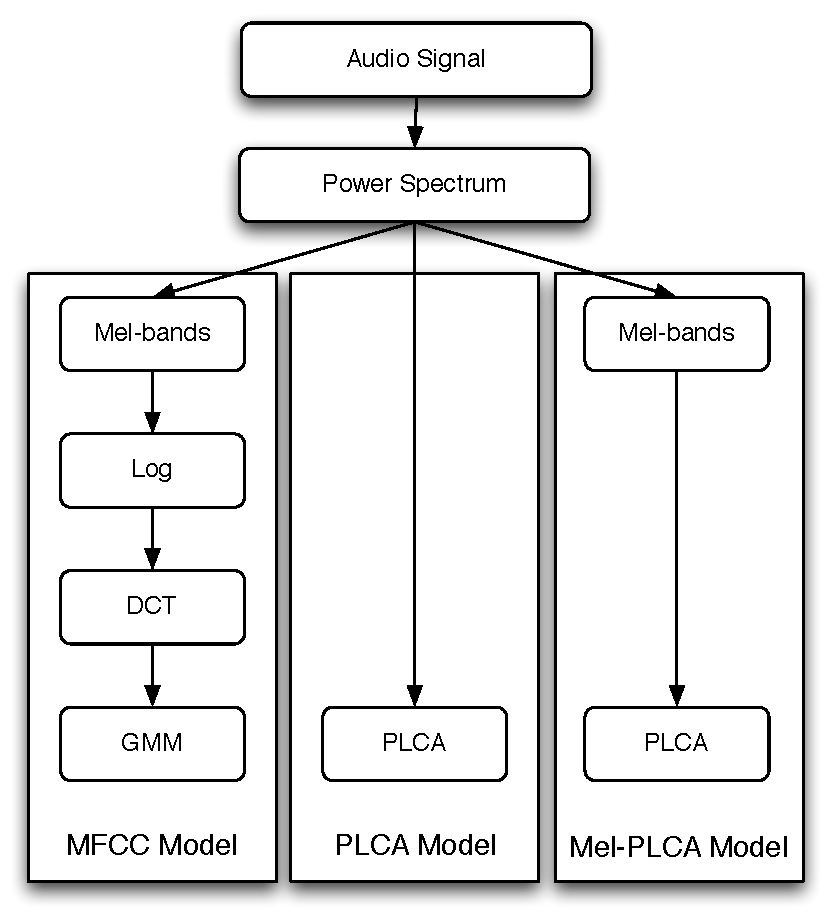
\includegraphics[width=0.99\textwidth]{images/models.pdf}
\caption{Overview of the different models}
\label{fig:models}
\end{figure}


We tested 3 kinds of models, (1), a Gaussian Mixture Model of Mel-Frequency Cepstral Coefficients (MFCC Model), (2), a probabilistic Latent Component Analysis of a frequency transformation (PLCA Model), and (3), a probabilistic Latent Component Analysis of a Mel-frequency transformation (Mel-PLCA Model).  In the following section, the models are explained in more detail.  The models are also summarized graphically in Figure \ref{fig:models}.

\subsubsection{MFCC model}
The first model we built describes each acoustic class by first decomposing each training example into a vector of Mel-frequency cepstral coefficients (MFCCs) and then building a classifier using a Gaussian Mixture Model (GMM).  

\paragraph{MFCCs}
The basic algorithm for computing MFCCs is summarized below:

\begin{enumerate}
\item Apply a Hanning window function to the input audio signal and take the discrete Fourier transform
\item Warp the absolute power spectrum into $M$ triangular sub-bands, spaced equally on the Mel-frequency scale with 50\% overlap.   The following approximate formula describes a frequency on the Mel-frequency scale given an input linear frequency:
\begin{equation}
mel(f) = 2595*\log_{10}{1+\frac{f}{700}}
\end{equation}
Use this mapping to warp the power spectrum to the Mel-scale and compute the energy in each sub-band as follows:
\begin{equation}
S_m = \log{\left(\sum_{k=0}^{N-1}|X[k]|^2H_m[k]\right)}
\end{equation}
where $H_m$ are the filter-banks described by the Mel-frequency scale.
\item Finally, after taking the $\log$ result, compute the discrete cosine transform to obtain the first $C$ MFCCs:
\begin{equation}
c_n = \sqrt{\frac{2}{M}}\sum_{m=1}^{M}(\log{S_m}\times\cos{[n(m-\frac{1}{2})]}\frac{\pi}{M}
\end{equation}
and $n = 1,...,C$, where $C$ is the number of coefficients to return (discarding high-frequency coefficients), and $M$ is the number of triangular sub-bands.
\end{enumerate}
 
\paragraph{GMM}

In order to describe our set of acoustic classes, we assumed the distribution of each class's MFCC vectors could be described by a multivariate Gaussian, i.e., for each class $k = {1...N}$, 
\begin{equation}
p(\mathbf{x}|k) \sim \mathcal{N}(\mu_{k}, \Sigma_{k})  
\end{equation}
where $\mu_{k}$ is the mean vector of MFCCs, and $\Sigma_{k}$ is the full covariance matrix.  In order to combine each of the $N$ classes into a mixture of Gaussians, we simply assumed a prior equal weighting on the mixture proportions of each Gaussian, i.e., $\pi_{k} = 1 / N$.  Finally, we assumed any test vector of MFCCs could be generated by one or more of the $N$ multivariate Gaussian distributions.  Classification was then calculated using the posterior probabilities $p(k|\mathbf{x})$ of each of the $k$ components in the Gaussian mixture distribution:

\begin{equation}
p(k|\mathbf{x}) = \frac{p(k)p(\mathbf{x}|k)}{\sum_{j}^{N}p(j)p(\mathbf{x}|j)}  
\end{equation}

\subsubsection{PLCA model}

As pLCA operates on a matrix in order to describe its latent decomposition, we first transposed each audio signal into a matrix describing the magnitude of frequencies over time.  Each audio signal was multiplied by a Hanning window and broken down into a frequency representation using the discrete Fourier transform with a window size of 371.5 ms (16384 samples at 44100 Hz), hop size of 92.9 ms (4096 samples at 44100 Hz).  Composing the absolute power spectrum into a matrix of frequency versus time denotes the Short Time Fourier Transform (STFT).

Using the formulation described in Section \ref{sec:plca}, we ran pLCA on each of the training example's STFT using a single component.  From these results, we formed a dictionary that was used for classification by aggregating into a matrix each class's latent frequency distribution, $p(f|k_i)$, for $i = {1...N}$ where $N$ equals the total number of trained classes.  Then, using the trained dictionary $p(f|k)$, the latent distribution over weights $p(k)$ and impulses $p(t|k)$ are maximized using the EM update rules described in Section \ref{sec:plca}.  As we were testing whether our possible distributions of frequencies (our dictionary) were capable of describing the audio signal, we did not allow updates of $p(f|k)$.

%Extending the model for Experiment 2, we define a dictionary with an additional randomly initialized component, and maximize the likelihood of each of the marginal distributions, allowing only the additional component to converge to a new distribution.  This ensures that either (1), the new frequency component is unnecessary to explain the observed data, and is effectively reduced to 0, or, (2), a new frequency component is necessary for explaining the data, and the new component is re-estimated to comprise the unexplained distribution of frequencies.  Effectively, this allows one to do denoising, where the components describing the dictionary are signal, and the unexplainable frequencies are projected in a new component defining the noise of the scene.  

%For experiment 3, we again train a single component as we do in Experiment 1 on each of the training examples.  Testing 

\subsubsection{Mel-PLCA Model}

The last model we describe was built in the same way as the PLCA model, except it uses as input a Mel-frequency transformed STFT rather than a linear-frequency scale (i.e. $p(f,t) \rightarrow p(S_m(f),t)$.  The Mel filter-bank effectively performs a data-reduction from a $16384$ point frequency transform in the standard PLCA model to a $40$ element vector by summing the energy in the Mel-frequency critical bands.  This model most resembles approaches taken in MPEG-7 Spectral Basis Decomposition, however does not take the last step of de-correlating the frequency scale, and further makes use of PLCA instead of PCA or ICA.  % It should be noted that in a preliminary investigation, we also tested a model using MFCCs as input to PLCA (MFCC-PLCA).  However, the performance of this model was as good as random and is therefore not reported here.

\subsection{Experiments}
\subsubsection{Experiment 1}
Most previous studies in acoustic classification use multiple examples of a single class in isolation.  However, as our investigation focused on classification performance during mixtures of classes, we only trained a single example of each class, building a set of 37 classifiers for experiment 1.  As a sanity check, we tested whether the MFCC and PLCA models were able to correctly classify the test example built using the 37 classifiers.

\subsubsection{Experiment 2}
For experiment 2, we determined whether the MFCC and PLCA models were able to correctly classify the trained class in the presence of an untrained class (noise).  As we have 37 classes, this equates to 36 possible mixtures for each class, where each of the 36 classes are trained in isolation, and tested in a mixture of a 37th untrained class.  In order to create the $37*36 = 1332$ possible mixtures, we used balanced mixing.  For this experiment, this means each class is actually represented with 36 possible examples (36 possible mixtures for each class).  

\subsubsection{Experiment 3}
For experiment 3, we added the 37th un-trained class to the set of possible classifiers in order to see if both classes could be correctly classified when presented as an acoustic mixture.  This means we tested on $37 \choose 2 = 666$ possible mixtures and sought to find out whether the MFCC and PLCA models were capable of classifying either or both of the mixed acoustic classes, even though they were presented as a single acoustic stream.


\subsection{Validation and Reporting}
\label{sec:ROC}
We performed k-fold cross-validation using 10-folds.  With 10 seconds per class (370 seconds total), this equates to 1 second folds per class where training occurs on 9 seconds of material per class, and testing occurs on 1 second of material per example. The results of all folds were then averaged together to produce a single estimation.

In order to assess the estimated results, we made use of a standard technique in describing classification performance, the Receiver Operator Characteristic (ROC) curve.  ROC analysis describes ground truth classes as true and false and the predicted measures as positive and negative for a binary classifier.  The ROC curve then measures the accuracy of the classifier in separating the actual true class from the non-classes by relating the sensitivity, or the \textit{true positive rate}, against 1$-$specificity, or the \textit{false positive rate}.   In order to build the curve for a continuous classifier, the classifier's response must be converted to a set of binary classifiers by using equally spaced thresholds.  We did this by taking equally spaced thresholds on the results of our cross-validation, and calculating the true positive rate of a bin $i$ as: 

\begin{equation}
TPR_i = \frac{TP}{TP + FN}
\end{equation}

and the false positive rate as: 

\begin{equation}
FPR_i = \frac{FP}{TN + FP}
\end{equation}

The resulting $(x,y)$ points relating the false positive rate to the true positive rate are plotted for each classifier.

A perfect score is denoted by 100\% sensitivity (no false negatives) and 100\% specificity (no false positives) and corresponds to a point in the top-left corner, (0,1).  A classifier that performs at chance lies along the diagonal going from the bottom-left to the top-right corner.  

As well, the area under the ROC curve (AUC) neatly summarizes the performance of the curve with 1.0 being a perfect score, and 0.5 being a classifier that performs at chance.  We can also understand the AUC as the probability of classifying a randomly chosen positive instance with higher likelihood than a negative one.

\section{Results}

\subsection*{Experiment 1: Classifying isolated acoustic textures}

We tested the performance of a single class in isolation as a sanity check, and as we expected, the performance of the MFCC and PLCA models as determined by the ROC analysis are excellent, with an AUC of within 0.001 of perfect discrimination.

%performance during sound classification of 37 classes 
%	- handle different amplitudes
%	- microphone dynamics? 
%	- similar classes? 

%As we'd expect, the performance of both the MFCC and PLCA models perform with a perfect AUC.  

%GMM-MFCC: 98.4\%, PLCA-1c: 78.1\%

\subsection*{Experiment 2: Classifying acoustic textures in the presence of noise}

\begin{figure}
\centering
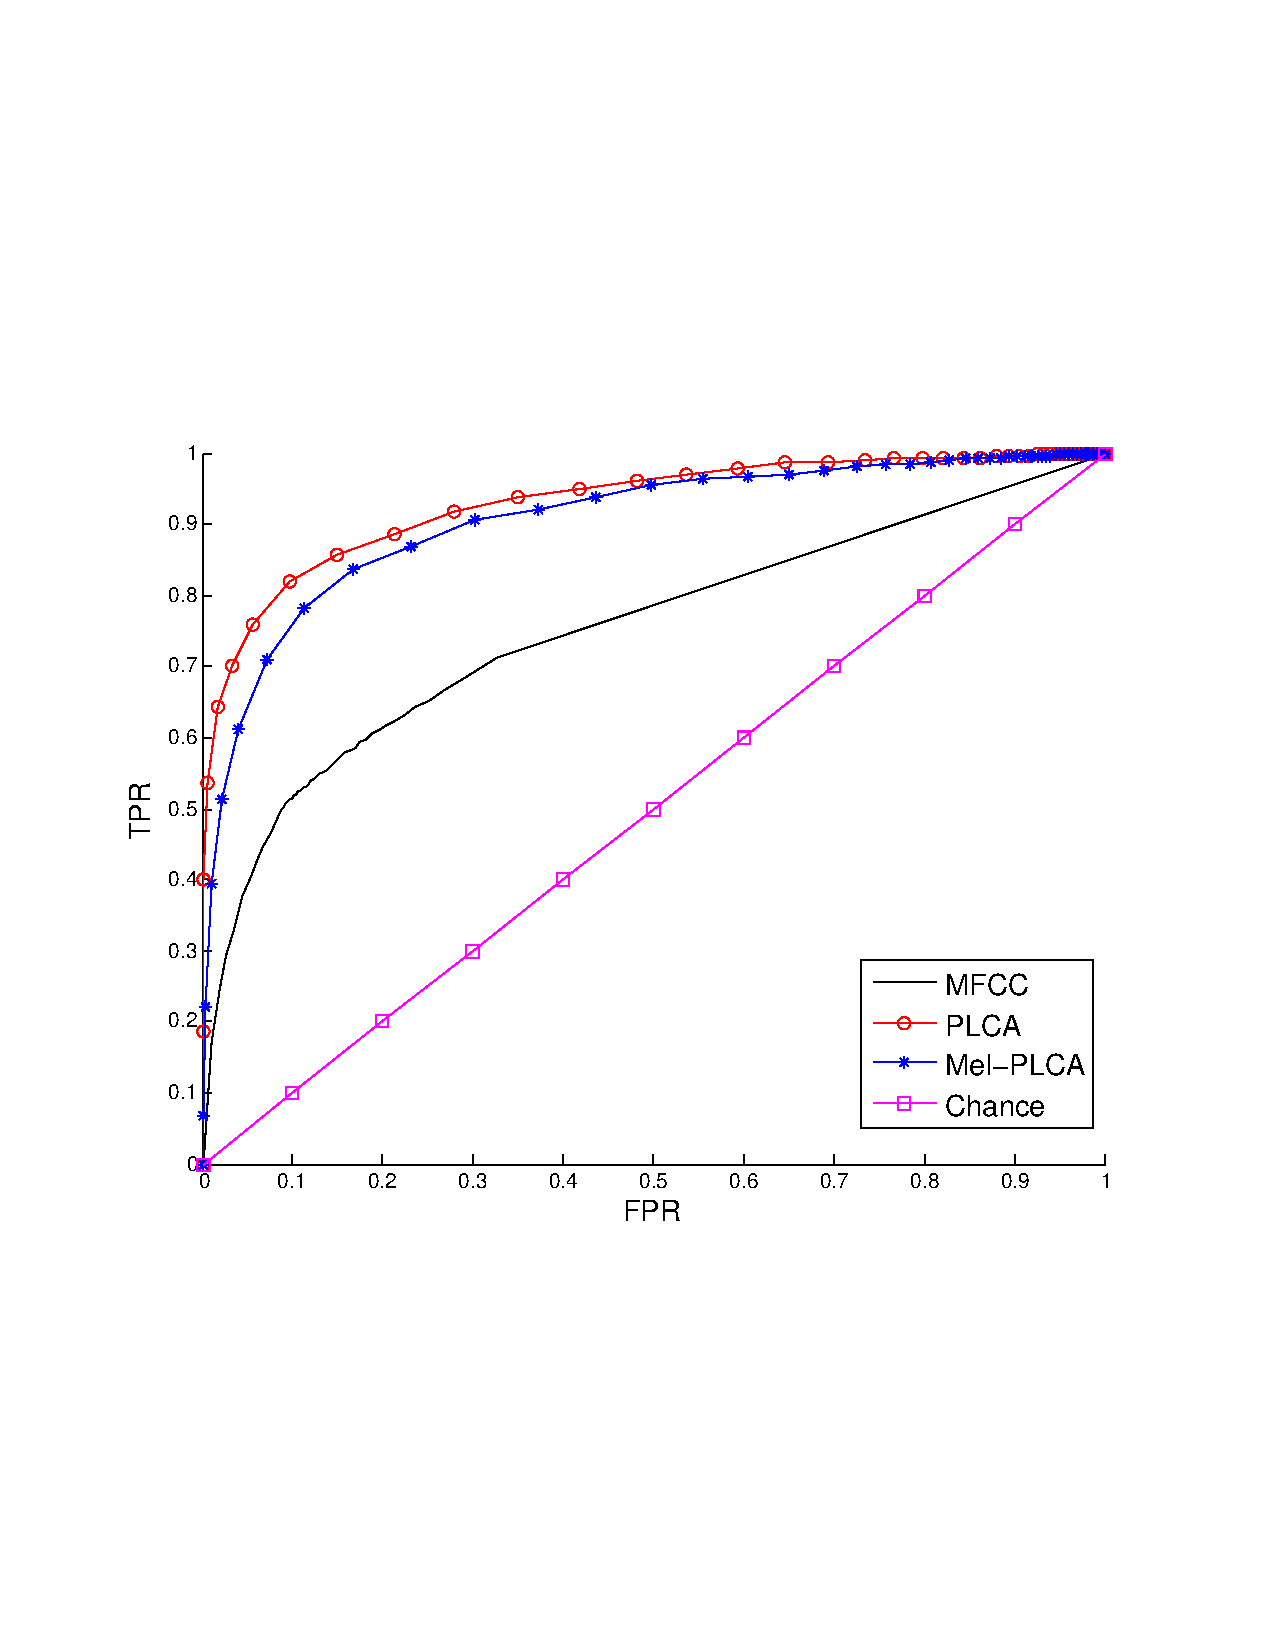
\includegraphics[width=0.99\textwidth]{images/unknown-mixture-roc-results.pdf}
\caption{Experiment 2: Classification masked by noise.}
\label{fig:unknown-mixture-roc-results}
\end{figure}

We tested the performance of both the MFCC and PLCA-based classifiers in the presence of noise by mixing one of 36 trained classes with an untrained class of sound (the 37th class), effectively masking the trained class with noise.  The average results of 1332 mixtures are depicted in Figure \ref{fig:unknown-mixture-roc-results} using ROC curves depicting each model's performance in classifying the correctly masked class.  We can see the MFCC model does well above chance, though both of the PLCA models do a far greater job.  Interestingly, the Mel-PLCA model is very close to the performance of the full-spectrum based PLCA model, even though this model uses only 40 samples versus 8192 samples per frequency frame.

\subsection*{Experiment 3: Classifying acoustic mixtures}


\begin{figure*}
\centering
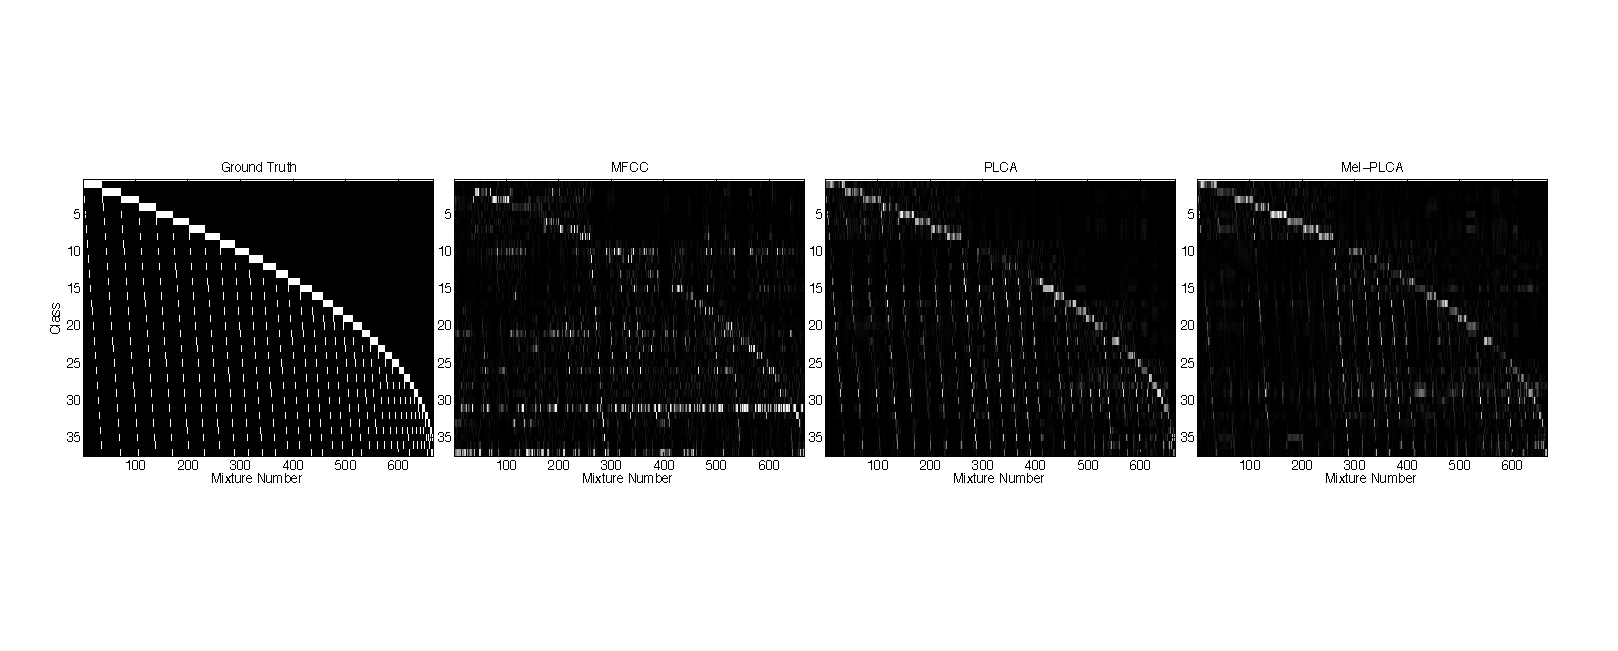
\includegraphics[width=0.99\textwidth]{images/mixture-img-results.pdf}
\caption{Experiment 3: Classification performance of acoustic mixtures depicting the ground truth classes for each of the 666 mixtures and the MFCC model, the PLCA model, and the Mel-PLCA model's classification likelihoods for each of the 666 mixtures. Images represent likelihood of a class in a given mixture, with white being 1.0, and black being 0.0.}
\label{fig:mixture-images}
\end{figure*}


\begin{figure}
\centering
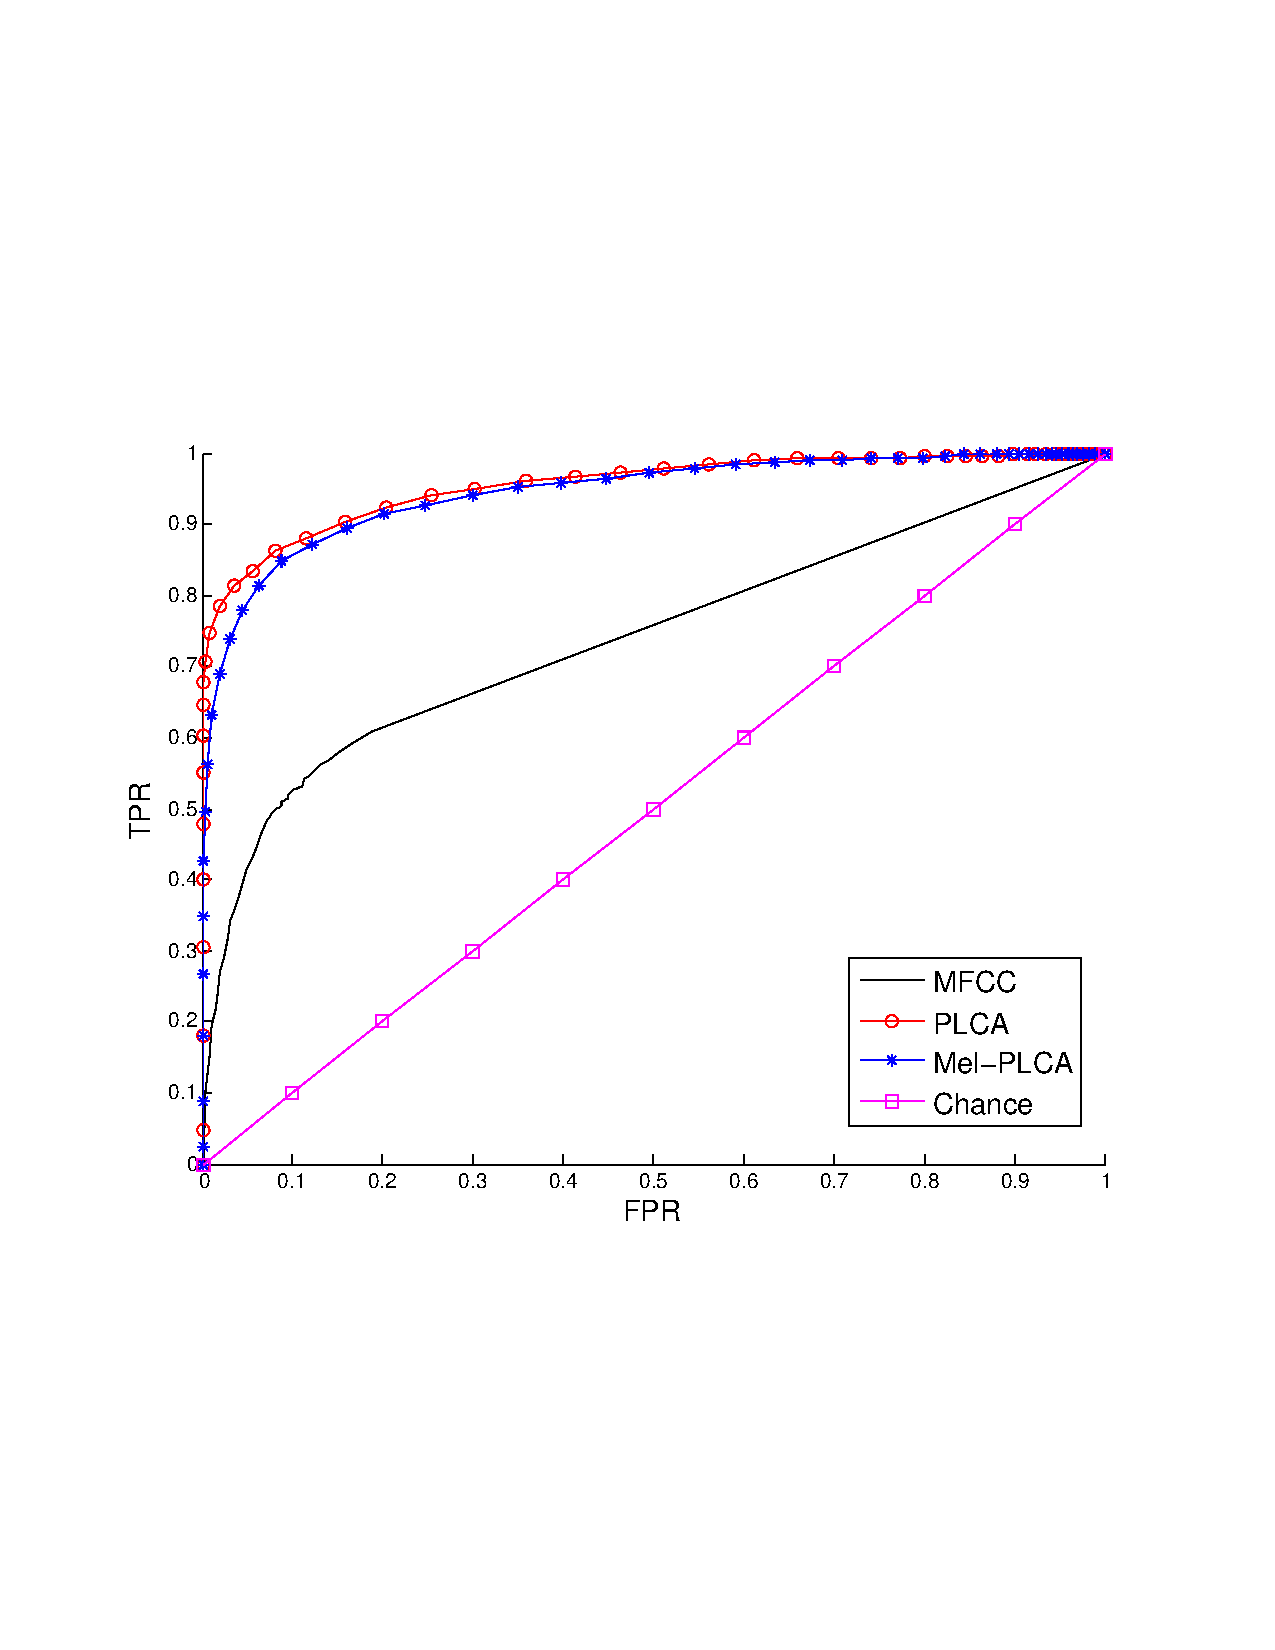
\includegraphics[width=0.99\textwidth]{images/mixture-roc-results.pdf}
\caption{Experiment 3: Classification of acoustic mixtures.}
\label{fig:mixture-roc-results}
\end{figure}



The last test we performed measures the performance of our 3 models to classify both classes in an acoustic mixture of 2.  The results depicted in Figure \ref{fig:mixture-images} show the ground truth for the 37 possible classes across all 666 mixtures ($37 \choose 2 = 666$ classes) as an image.  As well, this figure shows the likelihoods assigned to each of the 37 classes across all 666 mixtures for each of the 3 models.  From these figures, we can see the performance of the MFCC model struggles to classify most of the mixtures accurately, and often produces a false positive for classes 10 (conversation), 21 (laughing-man), and 31 (sword).  Thresholding columns of this image and storing the $TPR$ and $FPR$ as described in Section \ref{sec:ROC} produces 666 ROC curves.  The average of these curves are depicted in Figure \ref{fig:mixture-roc-results}, showing the performance of the MFCC model to be well above chance, though with the PLCA and Mel-PLCA models doing far better.  Interestingly again, we find the Mel-PLCA model is able to perform nearly as well as the PLCA model, performing within 0.01 of the PLCA model's AUC.  


\begin{table}
\centering
\caption{Area Under the Curve of ROC Analysis}
\begin{tabular}{|c|c|c|c|l|} \hline
Method&Experiment 1&Experiment 2&Experiment 3\\ \hline
MFCC&\textbf{1.0}&0.7388&0.7410\\ \hline
PLCA&\textbf{1.0}&\textbf{0.9303}&\textbf{0.9548}\\ \hline
Mel-PLCA&0.9989&0.9065&0.9443\\ \hline
\end{tabular}
\end{table}

%\subsection{Experiment 4}
%real-time on a mobile...

\section{Discussion}
\label{sec:discussion}

We tested the performance of 3 types of acoustic classification algorithms, 1 based on MFCCs and 2 based on pLCA.  All 3 models performed with excellent results when a single acoustic class appeared in isolation.  However, our interests were in how such models performed when classifying the \textit{parts} that make up an acoustic scene.  We therefore devised two additional experiments: Experiment 2 masked a known acoustic class by an unknown acoustic class, effectively adding noise; and Experiment 3 tested the performance of each model to classify multiple parts of an acoustic scene by mixing 2 classes together.  The MFCC model performed well above chance in both cases with an AUC of ~0.74, but the models built on pLCA performed with much stronger results, exhibiting > 0.9 AUC in both experiments.  

One possible reason for the poor performance of MFCCs during classification of mixtures is the signal model assumes a single excitation source (e.g. vocal tract or instrument).  In the presence of multiple sources then ambiguity is created, and it becomes difficult to estimate which source contributes to each of the coefficients, especially since the sources are also combined non-linearly through the step of a log-transformation. 

Two disadvantages of using a full and direct spectrum model such as our ``PLCA model'' noted by \cite{Casey2001a} is their inconsistency and dimensionality.  We therefore tested a second model similar to the MPEG-7 spectral basis decomposition described in  \cite{Casey2001a}, ``Mel-PLCA'', which reduced the 16384 point Fourier spectrum to a 40 element vector.  However, unlike the MPEG-7 spectral basis decomposition, we made 2 significant changes: (1) we make use of the Mel-frequency scale rather than log-decibel scaling and normalization; and (2), as the article in question was written nearly 12 years ago, the only basis methods described were SVD/ICA/ and PCA based methods as PLCA had not yet been published.  Incorporating these changes, we found that the Mel-PLCA model performed within 0.03 of the full-spectrum PLCA model.  Using the critical bands defined by the Mel-frequency scale ensures the inconsistencies that may be apparent within similar acoustic classes are averaged out, and perceptually relevant frequency dimensions describing the class are retained while keeping dimensionality very low.  

% The methods presented can be extended to do generalizable acoustic event classification by training multiple classifiers representative of the variety of events that describe each class.  However there are three issues with any solution based purely on frequency information.  First, there is a dependence on microphone responses.  As microphone responses create a filter on the frequencies able to be represented, determining events on a headset quality microphone using classifiers trained on a studio quality microphone will be very difficult.  Second, different compression rates will also affect the representation of frequency bands creating artificial banded filters.  Lastly, how sounds may be recorded will also create ``filters'' of sound that can affect the representation of frequencies describing a sound.  For instance, in comparison to sounds heard in front of a listener, sounds heard behind a listener have a ``low-pass'' filter on the frequency responses.  

\section{Future Work}

This work presents an early prototype of a broader framework capable of acoustic source separation and classification for content-based information retrieval.  A number of viable extensions are possible.  First, as we only made use of highly textured atmospheric sounds, it remains to be seen whether the following method alone would suffice in modeling more impulsive sounds, e.g. drums, birds, or less atmospheric sounds.  In such cases, an entropic prior on the temporal weights of a pLCA decomposition would very likely greatly improve results \cite{Smaragdis2007}, ensuring the sparsity of temporal weights in the latent distribution $p(t|k)$, while capturing the bulk of the frequency distribution in the latent factor $p(f|k)$. 

Second, 2D patch-based and shift-invariant convolutive pLCA \cite{Smaragdis2007} has shown great promise in capturing the structure of music when applied to chromagram features and when using sparsity and shift-invariance in all features \cite{Weiss2011}.  Such a technique has the power not just for classifying the instruments that describe a musical passage, but as well the course of events that describe the musical scene, essentially identifying whole musical passages or riffs.  

Third, In real-time scenarios, it is often the case that a dictionary of classes is not readily available.  Recent work describing the online-learning of dictionary elements using pLCA has shown great promise in performing real-time speech de-noising \cite{Duan2012}, resulting in components separating noise and speech.  Such a distinction has wide applications in fields such as surveillance and tele-presence technologies.  

Lastly, in developing this work, it became apparent that no standard publicly and freely available libraries for evaluating acoustic-based CBIR algorithms exists.  Though the problem is well noted in music information retrieval \cite{Casey2008b,Rhodes2010}, and recently addressed with databases such as the million song dataset \cite{Bertin-Mahieux2011}, no standardized databases have been developed as freely available archives in the general sound-based multimedia communities.  As such, testing the scalability of our approach proved very difficult, as we could only obtain 37 classes and a total of 1332 mixtures even though databases such as Youtube and typical multimedia archives are on the order of many millions.  Future work must therefore be done to help understand the scalability and performance across different approaches using a standardized database.  

